\section{建模过程（问题的量子化表示与转化方法）}
本文考虑的动力系统为 $40$ 维 Lorenz96：
\begin{equation}
\frac{dX_j}{dt} = (X_{j+1}-X_{j-2})X_{j-1} - X_j + F.
\end{equation}
观测模型写为
\begin{equation}
y_k = Hx_k + \varepsilon_k, \qquad \varepsilon_k \sim \mathcal{N}(0, R),
\end{equation}
其中 $H$ 为单位观测算子，观测噪声服从高斯分布。设集合规模为 $N_e$，第 $i$ 个状态维度对应的集合扰动向量记为 $\tilde{x}_i\in \mathbb{R}^{N_e}$，局地观测集合记为 $\mathcal{O}_i$，对应的观测扰动矩阵记为 $Y_i\in\mathbb{R}^{N_e\times |\mathcal{O}_i|}$。在经典 LETKF 中，若局地观测逆协方差为 $R_i^{-1}$，则权重空间的分析矩阵写为
\begin{equation}
C_i=\frac{N_e-1}{\lambda_{\mathrm{infl}}}I + Y_i R_i^{-1}Y_i^\top ,
\end{equation}
相应的均值权重与扰动变换矩阵为
\begin{equation}
\bar{w}_i=C_i^{-1}Y_iR_i^{-1}(y_i-\bar{y}_i),\qquad
W_i=\big((N_e-1)C_i^{-1}\big)^{1/2}.
\end{equation}
于是经典 LETKF 在第 $i$ 个维度上的分析均值与扰动分别为
\begin{equation}
\bar{x}^{a}_i=\bar{x}^{f}_i+\tilde{x}_i^\top \bar{w}_i,\qquad
\tilde{x}^{a}_i=\tilde{x}_i^\top W_i.
\end{equation}
本文所有修改都发生在 $R_i^{-1}$ 的构造以及 $\tilde{x}_i$ 的修正方式上，而不改变上述 LETKF 的基本权重空间框架。

为在受限量子资源下引入真实量子信息，本文不对整个 $40$ 维状态进行量子编码，而是将每个局地分析点附近的状态窗口与观测窗口提取为长度为 $4$ 的局地向量，再映射到 $4$ qubits 量子特征空间。设状态窗口为 $s_i$，观测窗口为 $o_j$，则它们经标准化后送入同一量子特征映射电路，得到两个量子态 $\lvert \phi(s_i)\rangle$ 与 $\lvert \phi(o_j)\rangle$。二者之间的量子相似度定义为
\begin{equation}
k_q(i,j)=|\langle \phi(s_i)\mid \phi(o_j)\rangle|^2 .
\end{equation}
该量子相似度反映了局地状态模式与观测模式之间的几何匹配程度。随后，我们不将其直接作为主导权重，而是与经典距离先验结合，构造成弱融合观测权重：
\begin{equation}
w_{ij}\propto \rho_{ij}\big((1-\lambda_\rho)+\lambda_\rho k_q(i,j)\big),
\end{equation}
其中 $\rho_{ij}$ 为经典距离先验，本文按
\begin{equation}
\rho_{ij}\propto 0.1+\exp\!\left(-\frac{d(i,j)^2}{2\sigma^2}\right),\qquad \sigma=\max(r/2,1),
\end{equation}
构造，并在局地窗口内重新归一化为均值为 $1$ 的权重。于是局地观测逆协方差被替换为
\begin{equation}
R_i^{-1}=\mathrm{diag}\!\left(\frac{w_{ij}}{\sigma_{\mathrm{obs}}^2}\right)_{j\in\mathcal{O}_i}.
\end{equation}
这一步清楚表明，本文不是替换 LETKF 的主体公式，而是替换了局地观测加权进入公式的那一层。

这种转化方式的关键意义在于，它把高维状态空间中的复杂建模问题，拆解成一系列局地窗口上的几何匹配问题。量子模块由此不再承担“直接求解全局最优状态”的角色，而是承担“为经典同化器提供局地结构线索”的角色。这种角色转化既符合赛题的量子资源约束，也使量子模块的物理解释更明确。

这里的“局地窗口”并不是单纯为了降维而做的技术处理，而是整个建模思路的核心。Lorenz96 本身具有明显的局地耦合结构，单个状态维度的演化主要受邻近维度影响。因此，如果把整个 $40$ 维状态一次性量子化，不仅资源上不可行，也会掩盖问题本来就具有的局地结构特征。相反，把问题拆解为多个重叠局地窗口后，每个窗口都可以被解释为一个小尺度的“状态模式识别”任务，量子模块在这里更容易发挥几何表示能力。

从建模角度看，本文的关键不是把经典变量机械映射到量子比特上，而是先完成一个问题重述：原问题是“如何在全局状态空间中更新分析场”，重述后变为“如何在每个局地窗口中识别哪些观测模式与当前状态更匹配”。量子特征映射承担的就是这个局地模式识别任务。这样一来，量子模块的输出不再是直接替代分析值，而是为后续的经典更新提供一张局地相似度地图。

\begin{figure}[htbp]
\centering
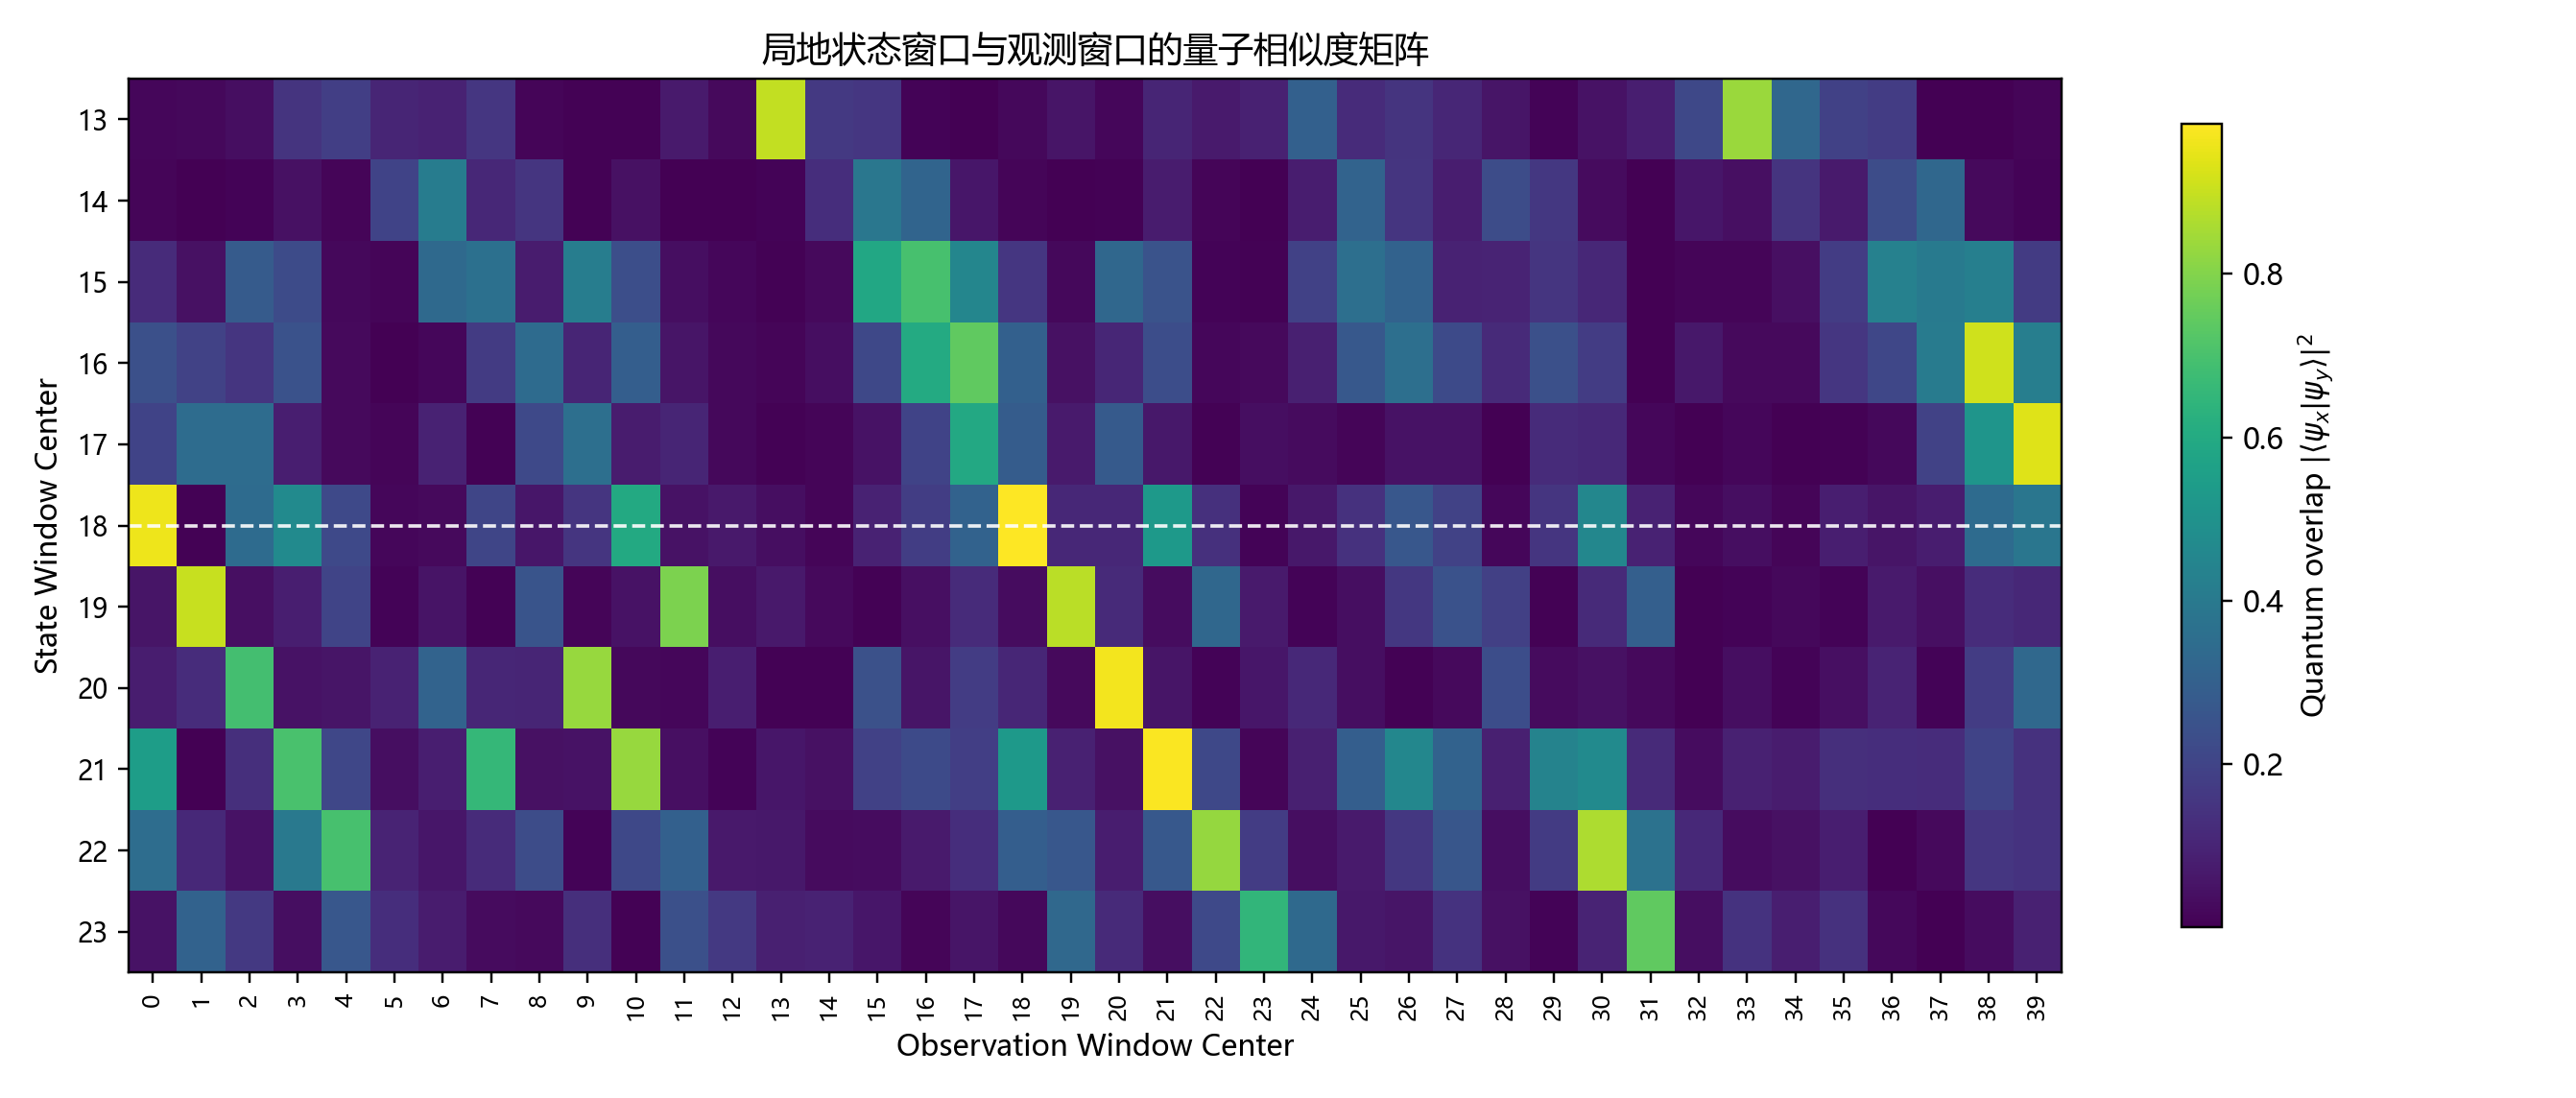
\includegraphics[width=0.92\linewidth]{figures/exp37_quantum_similarity_matrix.png}
\caption{代表性时间步下局地状态窗口与观测窗口之间的量子相似度矩阵。}
\label{fig:qsim}
\end{figure}

图 \ref{fig:qsim} 就是这种建模思想最直接的证据。若量子特征映射只是形式化编码，那么相似度矩阵应当接近随机噪声，缺乏清晰结构；而图中可以看到，相似度在不同窗口之间呈现出明显的强弱差异和局部团块结构。这说明量子特征映射确实捕捉到了状态窗口与观测窗口之间的非平凡几何关系。

更进一步看，图 \ref{fig:qsim} 还有两个重要含义。第一，它说明量子模块提供的不是一个全局统一系数，而是一张随窗口位置变化的结构图谱，这为后续局地加权提供了细粒度依据。第二，它也解释了为什么量子信息不宜直接做全局主导更新：这种相似度本来就是局地的、相对的、随时间变化的，如果把它直接放大到全局公式中，很容易造成过强扰动。因此，本文采用的弱融合建模其实并不是保守妥协，而是对量子相似度性质的自然响应。

除权重修正外，本文还对集合扰动方向引入一个弱 $J$ 修正。设量子权重归一化后得到 $q_i\in \mathbb{R}^{|\mathcal{O}_i|}$，则局地观测模式定义为
\begin{equation}
m_i=\frac{Y_i q_i-\mathrm{mean}(Y_i q_i)\mathbf{1}}{\|Y_i q_i-\mathrm{mean}(Y_i q_i)\mathbf{1}\|_2+\varepsilon}.
\end{equation}
再定义局地耦合系数
\begin{equation}
c_i=\frac{\langle \tilde{x}_i,m_i\rangle}{\|\tilde{x}_i\|_2+\varepsilon},
\end{equation}
并据此构造
\begin{equation}
J_i=c_i m_i,\qquad \tilde{x}_i^{(J)}=\tilde{x}_i+\lambda_J J_i .
\end{equation}
当前 exp37 受控实验并未额外引入硬门控阈值，等价于取门控变量 $g_i\equiv 1$；修正强度完全由 $c_i$ 与 $\lambda_J$ 决定。这一点需要特别说明，因为本文后续只讨论当前实验脚本对应的弱修正版本，而不把后续 gated 变体混入同一组结果表中。

因此，最终用于分析更新的公式为
\begin{equation}
\bar{x}^{a}_i=\bar{x}^{f}_i+(\tilde{x}_i^{(J)})^\top \bar{w}_i,\qquad
\tilde{x}^{a}_i=(\tilde{x}_i^{(J)})^\top W_i.
\end{equation}
基于上述分析，本文的建模过程可以概括为三步：首先利用 Lorenz96 的局地耦合结构把高维问题分解为多个局地窗口；其次在每个窗口上通过量子特征映射构造状态--观测相似度；最后再以“弱加权 + 弱方向修正”的方式把量子结构送入 LETKF。这样得到的模型既保留了经典同化的稳定性，也使读者能够明确看到本文相对于经典基线到底改动了哪一层、如何改动以及为什么必须弱改动。
